\subsection{\textit{Large-Scale Provisioning of
    Resource Constrained
    IoT Deployments, LEONORE}}
Riset dilakukan oleh Michael Vogler, Johannes M. Schleicher, Christian Inzinger, Stefan Nastic, Sanjin Sehic and Schahram Dustdar dari Vienna University of Technology. Riset ini menjelaskan mengenai cara pembuatan sebuah infrastruktur untuk melakukan \textit{provisioning} perangkat \textit{IoT} dalam skala besar. Penelitian ini berfokus untuk membuat sebuah pendekatan terstruktur dalam menyediakan layanan deployment lingkungan IoT dengan dua metode yaitu Push dan Pull.

Arsitektur dibuat dengan membuat 4 API yang dapat diakses oleh mulai dari  \textit{User API, Repository API, Device API, serta Provisioning}. Arsitektur ini memilki cara kerja yaitu menyimpan seluruh image atau dapat disebut sebagai deployment plan pada \textit{repository}, apabila repository membutuhkan dependency lain maka akan diletakan pada bagian \textit{artifact}. Artifact dibuat dan di proses oleh \textit{package builder} yang seluruh \textit{resources} nya diatur oleh komponen manajemen yaitu \textit{package, dependency management serta gateway management}. Setelah siap untuk di\textit{deploy}, bagian \textit{iot gateway handler} melakukan provisioning kepada target \textit{device}. Secara umum arsitektur leonore dapat dilihat pada gambar \ref{fig:arsitektur-leonore}

\begin{figure}[ht]
  \centering
  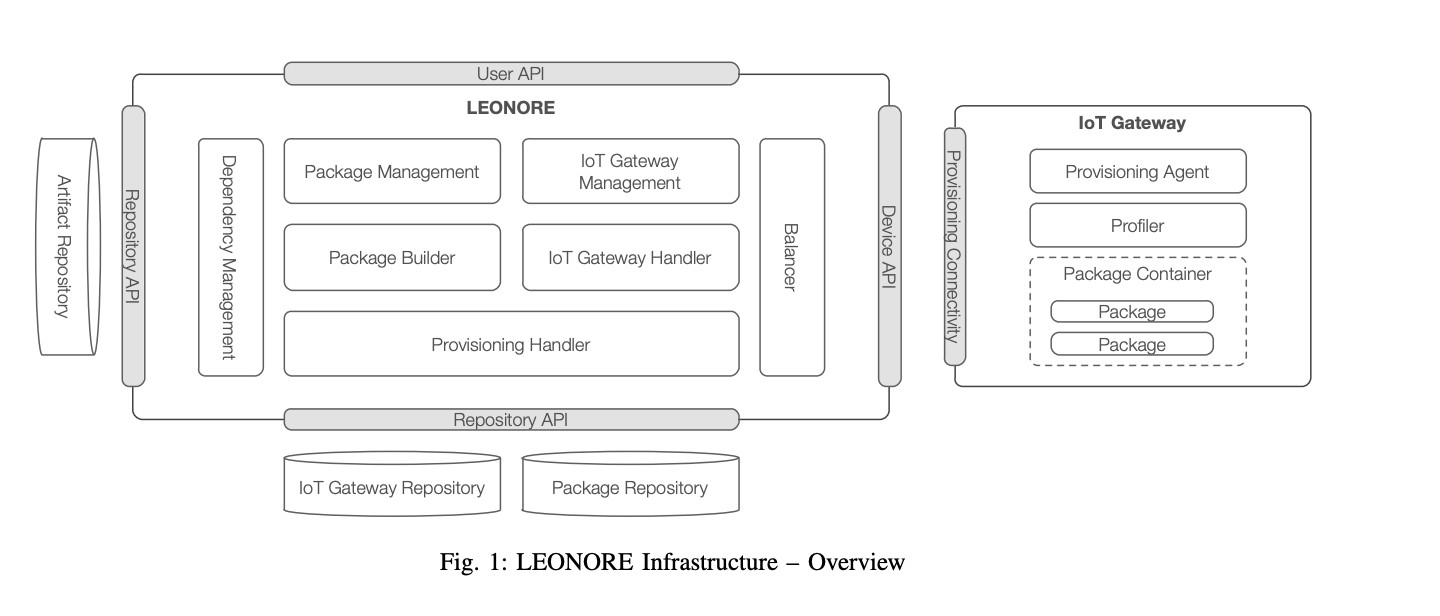
\includegraphics[width=0.8\textwidth]{resources/chapter-2/arsitektur-leonore.jpg}
  \caption{Arsitektur Leonore}
  \label{fig:arsitektur-leonore}
\end{figure}
% Penelitian ini telah diuji dalam skenario industri skala besar dunia nyata yaitu 1000 IoT Gateways yang tersebar di 10 yang memiliki 8 nodes dan masing masing 125 containers.